\section{Requirements Validation}
\begin{figure}[!h]
	\centering
	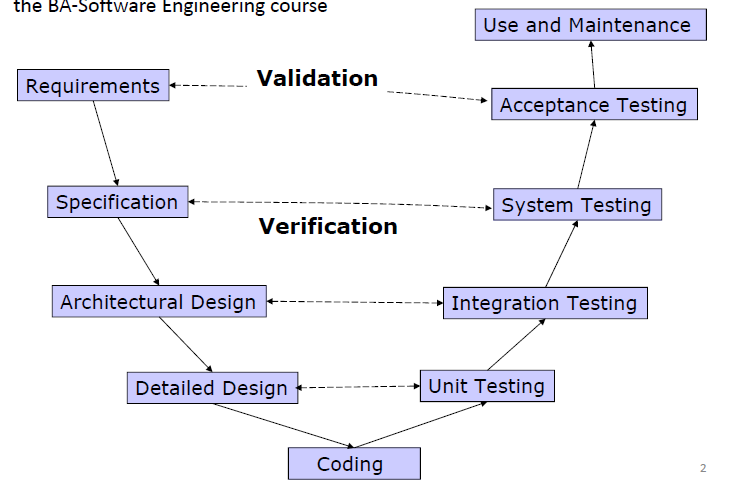
\includegraphics[scale=0.7]{img/v_modell.png}
\end{figure}

\begin{table}[!h]
	\begin{tabular}{|p{20em}|p{20em}|}
		\hline
		\textbf{Validation}	& \textbf{Verifikation}\\
		\hline
		Bauen wir das richtige System? & Bauen wir das System richtig?\\
		\hline
		Matcht die Problembeschreibung dem realen Problem?	& Entspricht Entwurf der Spezi?\\
		\hline
		Alle Bedürfnisse der Stakeholder erfasst? & Entspricht Implementierung der Spezi?\\
		\hline
		& Macht das fertige System auch genau das was wir sagen?\\
		\hline
		& Sind die R Models untereinander konsistent?\\
		\hline
	\end{tabular}
\end{table}

\begin{figure}[!h]
	\centering
	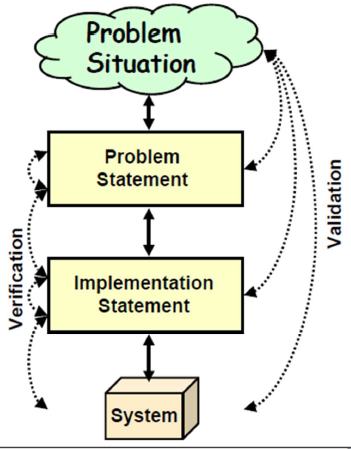
\includegraphics[scale=0.7]{img/verification_and_validation.png}
\end{figure}

\begin{figure}[!h]
	\centering
	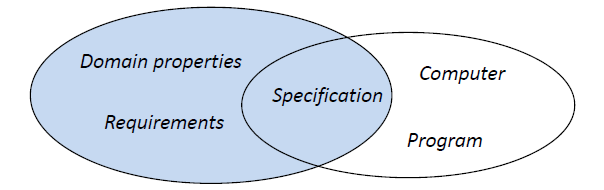
\includegraphics[scale=0.7]{img/re_world_other.png}
	\caption{Andere Darstellung der \ref{re_world}}
\end{figure}

\textbf{Domain Properties:} Dinge in der Anwendungsdomäne die wahr sind\\
\textbf{Requirements:} Dinge in der Anwendungsdomäne die wahr 'gemacht werden sollen' {\tiny RIP german..}\\
\textbf{Specification:} Beschreibung des Verhaltens damit Programm die R erfüllen kann\\
\\
\textbf{Zwei Verifikationskriterien}\\
- Programm, das auf Computer läuft, erfüllt die Spezifikation\\
- Spezifikation erfüllt die Requirements, bezogen auf die Domain Properties\\
\\
\textbf{Zwei Validierungskriterien}\\
- Haben wir alle wichtigen R aufgedeckt und auch verstanden?\\
- Haben wir alle wichtigen Domain Properties aufgedeckt und auch verstanden?\\
\\
Requirements Validation ist schwer, weil a) (philosophischer Natur) betrifft die Frage was ist wahr und erkennbar (knowable) und \\
b) (sozialer Natur) betrifft die Schwierigkeit einen Konsens zw Stakeholdern mit unterschiedlichen Zielen/Interessen zu finden.

\subsection{Validation Techniken}
\begin{itemize}
	\item Review
	\begin{itemize}
		\item Walkthrough\\
		verschiedene Rollen
		\begin{itemize}
			\item Review Leader\\
			Führt das Meeting; sorgt für fertige Vorbereitung ; erstellt Ergebnisbericht
			
			\item Recorder\\
			hält auftretende Issues fest
			
			\item Reader (meist der Autor)\\
			präsentiert Produkt Schritt für Schritt
			
			\item other reviewers
		\end{itemize}
		
		\item Inspection
		\begin{itemize}
			\item durchgeführt von Reviewern (und nicht dem Autor) 
			
			\item Vorbereitung: Reviewer inspizieren zunächst jeder für sich
			
			\item Collection Meeting: Reviewer treffen sich und gleichen Fehlerlisten ab
			
			\item nutzbare Rollenverteilung\\
			Round Robin: rundherum - Reviewer an der Reihe > vorstellen eines Issues\\
			Speed Review: jeder bekommt 3 Minuten zum darstellen seiner Ergebnisse
			
			\item benutze Checkliste mit Fragen/Issues
		\end{itemize}
	\end{itemize}
	
	\item Modellanalyse\\
	Modellanimation\\
	Begründung für Konsequenzen bestimmter R\\
	Begründung für Effekte von mgl Änderungen
	
	\item Meetings + regelmäßige Treffen mit Stakeholdern
	
	\item Prototyping
	\begin{figure}[!h]
		\centering
		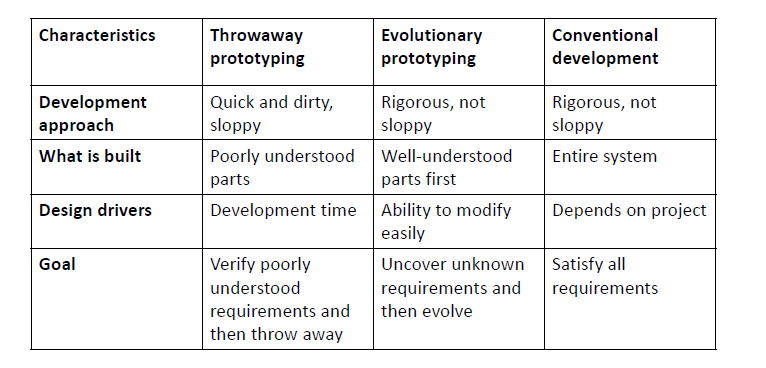
\includegraphics[scale=0.7]{img/prototyping_overview.png}
	\end{figure}
\end{itemize}

\subsection{A Constructive Approach for Design Space Exploration}
\begin{figure}[!h]
	\centering
	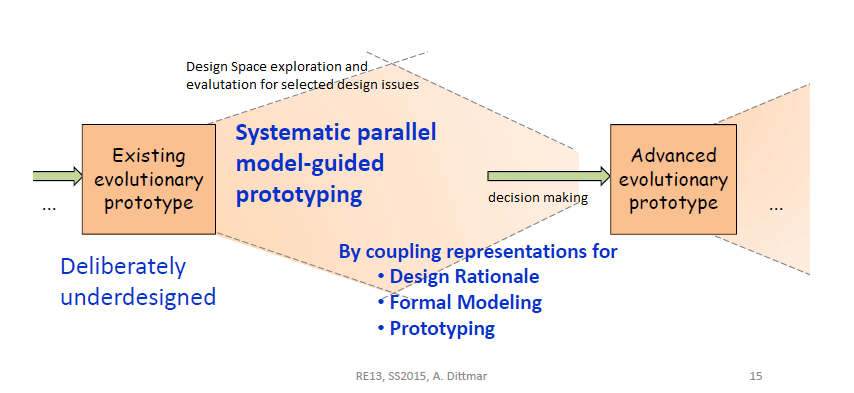
\includegraphics[scale=0.7]{img/constructive_approach.png}
	\caption{A Constructive Approach for Design Space Exploration}
\end{figure}
	

\begin{itemize}
	\item Design Rationale: QOC Notation
	
	\item Formal Modeling: HOPS Formalismen (Higher-order Processes Specification)
	\begin{itemize}
		\item HOPS Modelle verbinden QOC Diagramme und modellgetriebene Erweiterungen des existierenden evolutionären Prototyps\\
		mgl, weil: HOPS Prozesse können zusammengesetzt werden; können auf Java Klassen gemappt werden; HOPS Modelle können von HOPS Tools animiert werden
		
		\item einheitliche Beschreibung von Verhalten und strukturierten Aspekten eines interaktiven Teilsystems
			
		\item Essentielle Modeling Konzepte:\\
		Prozesse; Operationen; Teilprozesse; Komponenten
		
		\item Verteilte Beschreibung der Kontrolle
		
		\item Mapping von HOPS Prozessen auf Java Klassen
		
		\item Tool support
	\end{itemize}
	\textbf{Q-Models:} HOPS Models kontrollieren Apskete des Prototypen, die sich auf offene Fragen (Q) beziehen\\
	\textbf{O-Models:} HOPS Models für Optionen (O) um alternative Lösungen zu spezifizieren und modellgetriebenes Prototyping zu ermöglichen\\
	\textbf{C-Models:} HOPS Models für Kriterien (C)
	\begin{figure}[!h]
		\centering
		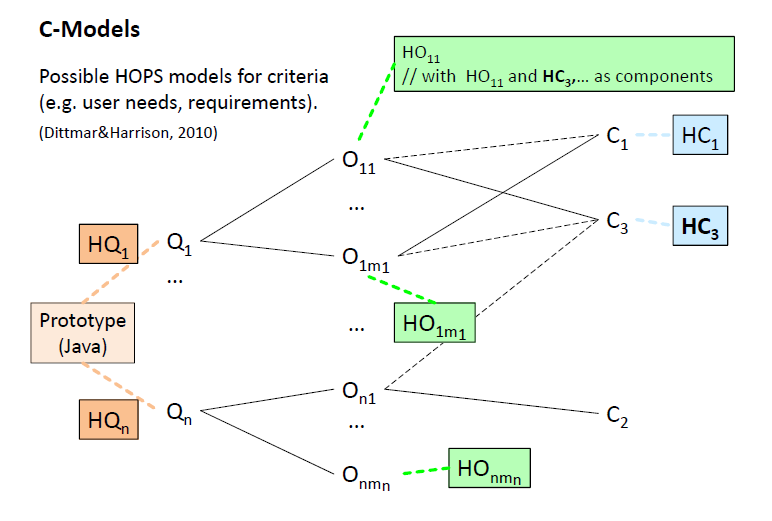
\includegraphics[scale=0.7]{img/hops_models_qoc.png}
		\caption{Nutzen von HOPS in QOC}
	\end{figure}
	\newpage
	\item Prototyping: Java
	
	\item Systematic Parallel Model-Guided Prototyping\\
	Plan für Zusammenführung von QOC-Modellen, HOPS-Modellen uind Implementierungen (JAVA)
	\begin{figure}[!h]
		\centering
		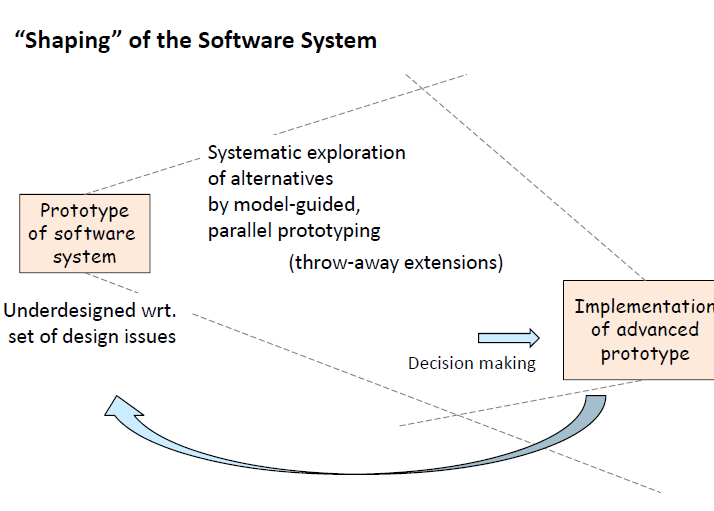
\includegraphics[scale=0.7]{img/shaping_system.png}
	\end{figure}
\end{itemize}

\newpage
\subsubsection{Summary}
\begin{itemize}
	\item Softwaresystem entwickelt sich Stück für Stück; Integration von evolutionärem und explorativem Prototyping
	
	\item Constructive Design Space Exploration: Verknüpfen von analytischen, empirischen und Implementierungs-Aktivitäten durch Evolution der Prototypen, formale Modelle
\end{itemize}


\subsection{Management of Requirements}
\textbf{Program Types}
\begin{itemize}
	\item \textbf{S-Programs} (specificable)\\
	Problem kann formal in einer Menge von Spezifikation beschrieben werden; verständliche Lösungen; geringe Änderungen notwendig
	
	\item \textbf{P-Programs} (problem solving)\\
	iterativer Prozess notwendig um Problem zu beschreiben und eine gute Lösung zu finden\\
	Software entwickelt sich iterativ, weil Lösung verbessert wird oder real world sich ändert
	
	\item \textbf{E-Programs} (embedded) \\
	System modelliert reald-world Prozesse und wird Teil der Welt, das modelliert wird. Systeme sind evolutionär.
\end{itemize}

\textbf{Management of R}
\begin{itemize}
	\item Angemessenes Erarbeiten der R\\
	einzelne R sollten identifizierbar sein\\
	R Attribute zuweisen:
	\begin{itemize}
		\item Identifier
		\item Quelle
		\item Autor
		\item Creation Date
		\item Änderungsdatum
		\item Status (set, agreed, released, rejected...)
		\item Priorität
	\end{itemize}
	use of tools
	
	\item Priorisieren der R (must be/should be/nice-to-have)\\
	wie wichtig ist jede R für den Kunden?\\
	Kosten für die Impl?\\
	wie risikobehaftet ist der Versuch diese R zu bauen?
	
	\item Managing R Change\\
	Software Evolution ist unausweichlich\\
	\textit{Verfolgbarkeit }von R ist wichtig
	\begin{itemize}
		\item Backward Verfolgbarkeit: jede R referenziert auf vorherige Versionen/Quellen\\
		Rückwärts nachvollziehbar in allen Entwicklungsschritten
		\item Forward Verfolgbarkeit: Vor. jede R muss eindeutig identifizierbar sein (uniqueID)\\
		"Forwärts" nachvollziehbar für alle neuen Dokumente die in SRS auftauchen können\\
		
 	\end{itemize}
	zwei Ansätze damit lar zu kommen
	\begin{itemize}
		\item Inkrementelle Entwicklung\\
		kurze Entwicklungszyklen\\
		stabile R in einem Zyklus erreichen\\
		neue R in nächstem Zyklus abarbeiten
		
		\item Explizites Änderungsmanagement\\
		Configuration Management (R Version)\\
		Baselines (stabile Version des Dokuments oder Systems)\\
		Formaler Bestätigungsprozess für Änderungen in nächster Baseline
	\end{itemize}
\end{itemize}